%%%%%%%%%%%%%%
%% Run LaTeX on this file several times to get Table of Contents,
%% cross-references, and citations.

%% If you have font problems, you may edit the w-bookps.sty file
%% to customize the font names to match those on your system.

%% w-bksamp.tex. Current Version: Feb 16, 2012
%%%%%%%%%%%%%%%%%%%%%%%%%%%%%%%%%%%%%%%%%%%%%%%%%%%%%%%%%%%%%%%%
%
%  Sample file for
%  Wiley Book Style, Design No.: SD 001B, 7x10
%  Wiley Book Style, Design No.: SD 004B, 6x9
%
%
%  Prepared by Amy Hendrickson, TeXnology Inc.
%  http://www.texnology.com
%%%%%%%%%%%%%%%%%%%%%%%%%%%%%%%%%%%%%%%%%%%%%%%%%%%%%%%%%%%%%%%%

%%%%%%%%%%%%%
% 7x10
%\documentclass{wileySev}

% 6x9
\documentclass{wileySix}

\usepackage{graphicx}

%%%%%%%
%% for times math: However, this package disables bold math (!)
%% \mathbf{x} will still work, but you will not have bold math
%% in section heads or chapter titles. If you don't use math
%% in those environments, mathptmx might be a good choice.

% \usepackage{mathptmx}

% For PostScript text
\usepackage{w-bookps}

%%%%%%%%%%%%%%%%%%%%%%%%%%%%%%%%%%%%%%%%%%%%%%%%%%%%%%%%%%%%%%%%
%% Other packages you might want to use:

% for chapter bibliography made with BibTeX
% \usepackage{chapterbib}

% for multiple indices
% \usepackage{multind}

% for answers to problems
% \usepackage{answers}

%%%%%%%%%%%%%%%%%%%%%%%%%%%%%%
%% Change options here if you want:
%%
%% How many levels of section head would you like numbered?
%% 0= no section numbers, 1= section, 2= subsection, 3= subsubsection
%%==>>
\setcounter{secnumdepth}{3}

%% How many levels of section head would you like to appear in the
%% Table of Contents?
%% 0= chapter titles, 1= section titles, 2= subsection titles, 
%% 3= subsubsection titles.
%%==>>
\setcounter{tocdepth}{2}

%% Cropmarks? good for final page makeup
%% \docropmarks

%%%%%%%%%%%%%%%%%%%%%%%%%%%%%%
%
% DRAFT
%
% Uncomment to get double spacing between lines, current date and time
% printed at bottom of page.
% \draft
% (If you want to keep tables from becoming double spaced also uncomment
% this):
% \renewcommand{\arraystretch}{0.6}
%%%%%%%%%%%%%%%%%%%%%%%%%%%%%%

%%%%%%% Demo of section head containing sample macro:
%% To get a macro to expand correctly in a section head, with upper and
%% lower case math, put the definition and set the box 
%% before \begin{document}, so that when it appears in the 
%% table of contents it will also work:

\newcommand{\VT}[1]{\ensuremath{{V_{T#1}}}}

%% use a box to expand the macro before we put it into the section head:

\newbox\sectsavebox
\setbox\sectsavebox=\hbox{\boldmath\VT{xyz}}

%%%%%%%%%%%%%%%%% End Demo


\begin{document}


\booktitle{Survey Methodology}
\subtitle{This is the Subtitle}

\authors{Robert M. Groves\\
\affil{Universitat de les Illes Balears}
Floyd J. Fowler, Jr.\\
\affil{University of New Mexico}
}

\offprintinfo{Survey Methodology, Second Edition}{Robert M. Groves}

%% Can use \\ if title, and edition are too wide, ie,
%% \offprintinfo{Survey Methodology,\\ Second Edition}{Robert M. Groves}

%%%%%%%%%%%%%%%%%%%%%%%%%%%%%%
%% 
\halftitlepage

\titlepage


\begin{copyrightpage}{2007}
Survey Methodology / Robert M. Groves . . . [et al.].
\       p. cm.---(Wiley series in survey methodology)
\    ``Wiley-Interscience."
\    Includes bibliographical references and index.
\    ISBN 0-471-48348-6 (pbk.)
\    1. Surveys---Methodology.  2. Social 
\  sciences---Research---Statistical methods.  I. Groves, Robert M.  II. %
Series.\\

HA31.2.S873 2007
001.4'33---dc22                                             2004044064
\end{copyrightpage}

\dedication{To my parents}

\begin{contributors}
\name{Masayki Abe,} Fujitsu Laboratories Ltd., Fujitsu Limited, Atsugi,
Japan

\name{L. A. Akers,} Center for Solid State Electronics Research, Arizona
State University, Tempe, Arizona

\name{G. H. Bernstein,} Department of Electrical and
Computer Engineering, University of Notre Dame, Notre Dame, South Bend, 
Indiana; formerly of
Center for Solid State Electronics Research, Arizona
State University, Tempe, Arizona 
\end{contributors}

\contentsinbrief
\tableofcontents
\listoffigures
\listoftables


\begin{foreword}
This is the foreword to the book.
\end{foreword}

\begin{preface}
This is an example preface.
This is an example preface.
This is an example preface.
This is an example preface.

\prefaceauthor{R. K. Watts}
\where{Durham, North Carolina\\
September, 2007}

\end{preface}


\begin{acknowledgments}
From Dr.~Jay Young, consultant from Silver Spring, Maryland, I received
the initial push to even consider writing this book. Jay was a constant
``peer reader'' and very welcome advisor durying this year-long process.


To all these wonderful people I owe a deep sense of gratitude especially now
that this project has been completed.
\authorinitials{G. T. S.}
\end{acknowledgments}

\begin{acronyms}
\acro{ACGIH}{American Conference of Governmental Industrial Hygienists}
\acro{AEC}{Atomic Energy Commission}
\acro{OSHA}{Occupational Health and Safety Commission}
\acro{SAMA}{Scientific Apparatus Makers Association}
\end{acronyms}

\begin{glossary}
\term{NormGibbs}Draw a sample from a posterior distribution
of data with an unknown mean and variance using Gibbs sampling.

\term{pNull}Test a one sided hypothesis from a numberically
specified posterior CDF or from a sample from the posterior

\term{sintegral}A numerical integration using Simpson's rule
\end{glossary}

\begin{symbols}
\term{A}Amplitude

\term{\hbox{\&}}Propositional logic symbol 

\term{a}Filter Coefficient

\bigskip

\term{\mathcal{B}}Number of Beats
\end{symbols}

\begin{introduction}

%% optional, but if you want to list author:

\introauthor{Catherine Clark, PhD.}
{Harvard School of Public Health\\
Boston, MA, USA}

The era of modern \index{microelectronics}\index{microelectronics!modern} 
began in 1958 with the invention of the
integrated circuit by J.~S.~Kilby
 of Texas Instruments \cite{kilby}.
His first chip is shown in Fig.~I. For comparison,
Fig.~I.2 shows a modern microprocessor chip, \cite{beren}.


This is the introduction.
This is the introduction.
This is the introduction.
This is the introduction.
This is the introduction.
This is the introduction.

\begin{equation}
ABC {\cal DEF} \alpha\beta\Gamma\Delta\sum^{abc}_{def}
\end{equation}


\begin{chapreferences}{3.}
\bibitem{zkilby}J. S. Kilby,
``Invention of the Integrated Circuit,'' {\it IEEE Trans. Electron Devices,}
{\bf ED-23,} 648 (1976).

\bibitem{zhamming}R. W. Hamming,
                 {\it Numerical Methods for Scientists and 
                 Engineers}, Chapter N-1, McGraw-Hill, 
                 New York, 1962.

\bibitem{zHu}J. Lee, K. Mayaram, and C. Hu, ``A Theoretical
               Study of Gate/Drain Offset in LDD MOSFETs''
                     {\it IEEE Electron Device Lett.,} {\bf EDL-7}(3). 152 
                     (1986).
\end{chapreferences}
\end{introduction}


\part[Submicron Semiconductor Manufacture]
{Submicron Semiconductor\\ Manufacture}

\chapter{Home}

\chapter{Overview}

\chapter{Environtment Setup}

\chapter{Basic Syntax}

\chapter{Variabel Type}

\chapter{Basic Operator}

\chapter{Desicion Making}

\chapter{Loop}

\chapter{Numbers}

\chapter{Strings}

\chapter{Lists}

\chapter{Tuples}

\chapter{Dictionary}

\chapter{Functions}

\chapter{Modules}

\chapter{Files I/O}

\chapter{Exceptions}

\chapter{Clasess/Object}

\chapter{Reg Expression}

\chapter{CGI Programming}

\chapter{Databases Access}
 
\chapter{Sending Email}

\chapter{Multithreading}
\section{Multithreading}
\hspace*{0.5in} Menjalankan beberapa\textit{ thread} mirip dengan menjalankan beberapa program yang berbeda secara bersamaan, namun dengan manfaat berikut : 

\begin{itemize}
\item Beberapa \textit{thread} dalam proses berbagi ruang data yang sama dengan benang induk dan karena dapat saling berbagi informasi atau berkomunikasi satu sama lain dengan lebih muda daripada jika prosesnya terpisah 

\item \textit{thread} terkadang disebut proses ringan dan tidak membutuhkan banyak memori atas, mereka lebih murah daripada proses
\end{itemize}

\hspace*{0.5in} Sebuah \textit{thread} memiliki permulaan, urutan eksekusi dan sebuah kesimpulan. Ini memiliki pointer perintah yang melacak dari mana dalam konteksnya saat ini berjalan:

\begin{itemize}
\item Hal ini dapat dilakukan sebelum pre-\textit{empted} (\textit{inturrepted})

\item Untuk sementara dapat ditunda sementara \textit{thread} lainnya yang sedang berjalan ini disebut unggul.
\end{itemize}
 
\subsection {Memulai Thread Baru} 
\hspace*{0.5in} Untuk melakukan \textit{thread} lain, perlu memanggil metode berikut yang tersedia dimodul \textit{thread} : 
\begin{center}{\fontsize{9pt}{9pt}\selectfont Thread.start $  \_  $new $  \_  $thread (function, args [, kwargs] )}
\end{center} 
\hspace*{0.5in} Pemanggilan metode ini memungkinkan cara cepat dan tepat untuk membuat \textit{thread} baru di linux dan window.Pemanggilan metode segera kembali dan anak  \textit{thread} dimulai dan fungsi pemanggilan dengan daftar \textit{args} telah berlalu. Saat fungsi kembali ujung \textit{thread} akan berakhir. Disini, \textit{args }adalah tupel argumen. Gunakan tupel kosong untuk memanggil fungsi tanpa melewati argumen. \textit{Kwargs} adalah kamus opsional argumen kata kunci.  
 
\vspace{12pt}
Contoh : 
\begin{verbatim}
\#  $!/usr/bin/python} 

Import thread
Import time

#  $ Define a function for the thread 
 
Def print $  \_  $time (threadNamw, delay):
   Count = 0
   While count <5:
   Time.sleep(delay)
   Count +=1 
   Print  $ " $ $  \%  $s :  $  \%  $s $ " $  $  \%  $ 
   (threadName, time.ctime(time.time()))
 
#  $ Create two thread as follows
try:
thread.start $  \_  $new $  \_  $thread(print $  \_  
$time, ( $ " $Thread-1 $ " $, 2, ))
thread.start $  \_  $new $  \_  $thread(print $  \_  
$time, ( $ " $Thread-2 $ " $, 4,))
except: 
print " $Error: unable to start thread 

while 1:
pass} 
\end{verbatim}

\vspace{80pt}
Bila kode diatas dieksekusi, maka menghasilkan hasil sebagai berikut : 
\vspace{10pt}
 
\begin{center}{\fontsize{10pt}{10pt}\selectfont Thread-1 : Thu Jan 22 15:42:17 2009}\end{center} 
 
\begin{center}{\fontsize{10pt}{10pt}\selectfont Thread-1 : Thu Jan 22 15:42:19 2009}\end{center} 
 
\begin{center}{\fontsize{10pt}{10pt}\selectfont Thread-2 : Thu Jan 22 15:42:19 2009}\end{center} 
 
\begin{center}{\fontsize{10pt}{10pt}\selectfont Thread-1 : Thu Jan 22 15:42:21 2009}\end{center} 
 
\begin{center}{\fontsize{10pt}{10pt}\selectfont Thread-2 : Thu Jan 22 15:42:23 2009}\end{center} 
 
\begin{center}{\fontsize{10pt}{10pt}\selectfont Thread-1 : Thu Jan 22 15:42:23 2009}\end{center} 
 
\begin{center}{\fontsize{10pt}{10pt}\selectfont Thread-1~:  Thu Jan 22 15:42:23 2009}\end{center} 
 
\begin{center}{\fontsize{10pt}{10pt}\selectfont Thread-1 : Thu Jan 22 15:42:25 2009}\end{center} 
 
\begin{center}{\fontsize{10pt}{10pt}\selectfont Thread-2 : Thu Jan 22 15:42:27 2009}\end{center} 
 
\begin{center}{\fontsize{10pt}{10pt}\selectfont Thread-2 : Thu Jan 22 15:42:31 2009}\end{center} 
 
\begin{center}{\fontsize{10pt}{10pt}\selectfont Thread-2 : Thu Jan 22 15:42:35 2009}\end{center} 

\vspace{12pt}
\hspace*{0.5in} Meskipun sangat efektif untuk benang tingkat rendah, namun modul \textit{thread} sangat terbatas dibandingkan dengan modul yang baru. 
\vspace{12pt}

\subsection{Modul Threading } 
\hspace*{0.5in} Modul threading yang lebih baru disertakan dengan Python 2.4 memberikan jauh lebih kuat, dukungan tingkat tinggi untuk \textit{thread}\textit{ }dari modul\textit{ }\textit{thread}\textit{ }dibahas pada bagian sebelumnya. The \textit{thread}\textit{ing }modul mengekpos semua metode dari \textit{thread}\textit{ }dan menyediakan beberapa metode tambahan : 

\begin{itemize}
\item \textbf{t}\textbf{hreading.activeCount() } 

Mengembalikan jumlah objek \textit{thread} yang aktif 
\item \textbf{t}\textbf{hreading.currentThread() } 

Mengembalikan jumlah objek \textit{thread} dalam kontrol benang pemanggil 
\item \textbf{t}\textbf{hreading.enumerate() } 

Mengembalikan daftar semua benda \textit{thread}\textit{ }yang sedang aktif 

\vspace{12pt}
\hspace*{0.5in} Selain metode, modul \textit{thread}\textit{ing }memiliki \textit{thread}\textit{ }kelas yang mengimplementasikan \textit{thread}\textit{ing. }Metode yang disediakan oleh \textit{thread}\textit{ }kelas adalah sebagai berikut : 
\item \textbf{run()} 

Metode adalah titik masuk untuk \textit{thread} 
\item \textbf{start()} 

Metode dimulai\textbf{ }\textit{thread}\textit{ }dengan memanggil metode run 
\item \textbf{join(}\textbf{[time]}\textbf{)} 

Menunggu benang untuk mengakhiri 
\item \textbf{isAlive()} 

Metode memeriksa apakah\textbf{ }\textit{thread}\textit{ }masih mengeksekusi\textbf{ } 
\item \textbf{getName()} 

Metode mengambalikan nama\textbf{ }\textit{thread} 
\item \textbf{setName()} 

Metode menetapkan nama\textbf{ }\textit{thread} 
\vspace{12pt}

\subsection {Membuat Thread Menggunakan Modul} 
\hspace*{0.5in} Mendefinisikan subclass dari \textit{thread} kelas, Menimpa  $  \_  $init $  \_  $ (self [args]) metode untuk menambahkan argumen tambahan 
, Menimpa run(self[args]) metode untuk menerapkan apa \textit{thread} harus dilakukan ketika mulai

\vspace{12pt}
\hspace*{0.5in} Setelah membuat baru \textit{thread} subclass, dapat membuah seuah instance dari itu dan kemudian memulai \textit{thread} baru dengan menerapkan \textit{start(),} yang ada gilirinnya panggilan \textit{run()} metode. 
\
vspace{12pt}
Contoh :
\begin{verbatim} 
#  $!/usr/bin/python
 
import threading
import time
 
exitFlag = 0
 
class myThread (threading.Thread): 
     def $  \_  $init $  \_  $(self, threadID, name, 
     counter) :
     threading.Thread. $  \_  $init $  \_  $(self)} 
     self.threadID = threadID
     self.name = name 
     self.counter = counter 
     def run (self) :
     print  $ " $Starting  $ " $ + self.name 
     print $  \_  $time(self.name, self.counter, 5)
     print  $ " $Exiting  $ " $+ self.name
 
def print $  \_  $time(threadName, delay, counter):} 

while counter:
 
     if exitFlag: 
     threadName.exit() 
     time.sleep(delay) 
     print  $ " $ $  \%  $s:  $  \%  $s $ " $  $  \%  
     $ (threadName, time.ctime(time.time()))
counter -= 1} 
 
#  $ Create new threads
thread1 = myThread(1,  $ " $Thread-1 $ " $, 1)
thread2 = myThread(2,  $ " $Thread-2 $ " $, 2)
#  $ Start new threads
thread1.start()
thread2.start()
print  $ " $Exiting Main Thread $ " $
\end{verbatim}

\vspace{12pt}
Ketika kode diatas dijalankan, menghasilkan hasil sebagai berikut:

{\fontsize{10pt}{10pt}\selectfont Starting Thread-1} 
 
{\fontsize{10pt}{10pt}\selectfont Starting Thread-2} 
 
{\fontsize{10pt}{10pt}\selectfont Exiting Main Thread} 
 
{\fontsize{10pt}{10pt}\selectfont Thread-1 : Thu Mar 21 09:10:03 2013} 
 
{\fontsize{10pt}{10pt}\selectfont Thread-1 : Thu Mar 21 09:10:04 2013} 
 
{\fontsize{10pt}{10pt}\selectfont Thread-2 : Thu Mar 21 09:10:04 2013} 
 
{\fontsize{10pt}{10pt}\selectfont Thread-1 : Thu Mar 21 09:10:05 2013} 
 
{\fontsize{10pt}{10pt}\selectfont Thread-2 : Thu Mar 21 09:10:06 2013} 
 
{\fontsize{10pt}{10pt}\selectfont Thread-1 : Thu Mar 21 09:10:07 2013} 
 
{\fontsize{10pt}{10pt}\selectfont Exiting Thread-1} 
 
{\fontsize{10pt}{10pt}\selectfont Thread-2 : Thu Mar 21 09:10:08 2013} 
 
{\fontsize{10pt}{10pt}\selectfont Thread-2 : Thu Mar 21 09:10:10 2013} 
 
{\fontsize{10pt}{10pt}\selectfont Thread-2 : Thu Mar 21 09:10:12 2013} 
 
{\fontsize{10pt}{10pt}\selectfont Exiting Thread=2} 

\vspace{10pt}
\subsection{Sinkronisasi Thread}
\hspace*{0.5in} \textit{T}\textit{hread}\textit{ing }modul disediakan dengan Python termasuk sederhana untuk menerapkan mekanisme bahwa memungkinkan untuk menyinkronkan \textit{thread}\textit{ }penguncian. Sebuah kunci baru dibuat dengan memanggil \textit{lock() }metode yang mengembalikan kunci baru. 
The \textit{acquire}\textit{ }\textit{(blocking)}\textit{ }metode objek kunci baru digunakan untuk memaksa \textit{thread}\textit{ }untuk menjalankan serempak. Opsional \textit{blocking} parameter memungkikan untuk mengontrol apakah\textit{ thread} menunggu untuk mendapatkan kunci. 
Jika \textit{blocking} diatur ke 0, \textit{thread} segera kembali dengan nilai 0 jika kunci tidak dapat diperoleh dan dengan 1 jika kunci dikuisisi. Jika pemblokiran diatur ke 1, blok dan menunggu kunci yang akan dirilis. 
The \textit{release()} metode objek kunci baru digunakan untuk melepaskan kunci ketika tidak lagi diperlukan.  
 
\vspace{12pt}
Contoh: 

\begin{verbatim}
#  $!/usr/bin/python
 
import threading
import time

class myThread (threading.Thread): 
   def $  \_  $init $  \_  $(self, threadID, name, 
   counter):
   threading.Thread. $  \_  $init $  \_  $(self)
   self.threadID = threadID
   self.name = name
   self.counter = counter
def run(self) 
   print  $ " $Starting  $ " $+ self.name 
   $  \#  $ Get lock to synchronize threads 
   ThreadLock.acquire() 
   print $  \_  $time(self.name, self.counter, 3) 
   #  $ Free lock to realease next thread
  ThreadLock.release()
Def print $  \_  $time(threadName, delay, counter):
   while counter:
   time.sleep(delay)
   print  $ " $ $  \%  $s:  $  \%  $s $ " $  $  \%  $ 
   (threadName, time.ctime(time.time()))
   counter -= 1
   threadLock = threading.Lock() 
   threads = []
#  $ Create new threads
thread1 = myThread(1,  $ " $Thread-1,1 ) 
thread2 = myThread(2,  $ " $Thread-2,2 )
#  $ Start new Threads} 
thread1.start() 
thread2.start()
 
#Add threads to thread list} 
threads.append(thread1)} 
thread2.append(thread2)} 
\vspace{10pt}
 
#  $ Wait for all threads to complete}  
Fort t in threads:
t.join()
print  $ " $Exiting Main thread $ " $
\end{verbatim}

\vspace{8pt}
Bila kode diatas dieksekusi, maka menghasilkan sebagai berikut : 

{\fontsize{10pt}{10pt}\selectfont Starting Thread-1} 
 
{\fontsize{10pt}{10pt}\selectfont Starting Thread-2} 
 
{\fontsize{10pt}{10pt}\selectfont Thread-1: Thu Mar 21 09:11:28 2013} 
 
{\fontsize{10pt}{10pt}\selectfont Thread-1: Thu Mar 21 09:11:29 2013} 
 
{\fontsize{10pt}{10pt}\selectfont Thread-1: Thu Mar 21 09:11:30 2013} 
 
{\fontsize{10pt}{10pt}\selectfont Thread-2: Thu Mar 21 09:11:32 2013} 
 
{\fontsize{10pt}{10pt}\selectfont Thread-2: Thu Mar 21 09:11:34 2013} 
 
{\fontsize{10pt}{10pt}\selectfont Thread-2: Thu Mar 21 09:11:36 2013} 
 
{\fontsize{10pt}{10pt}\selectfont Exiting Main Thread} 

\vspace{8pt}
\subsection{Multithreaded Antrian Prioritas} 
\hspace*{0.5in} The queue modul memungkinkan untuk membuat objek antrian baru yang dapat menampung jumlah tertentu item. Ada metode berikut untuk mengontrol antrian : 
\begin{itemize}
\item \textbf{get()} 

Menghapus dan mengembalikan item dari antrian
\item \textbf{put()} 

Menambahkan item ke antrian	
\item \textbf{qsize()} 
	
Mengembalikan jumlah item yang saat ini dalam antrian
\item \textbf{empty()} 

Mengembalikan benar jika antrian kosong jika tidak, salah
\item \textbf{full()}

Mengembalikan benar jika antrian penuh jika tidak, salah
\end{itemize} 

\vspace{12pt} 
Contoh:  
\begin{verbatim}
#  $!/usr/bin/python}  

import Queue
import threading
import time
 
exitFlag = 0 

class myThread (threading.Thread): 
def   $  \_  $init $  \_  $(self, threadID, name, q):
      threading.Thread. $  \_  $init $  \_  $(self) 
      self.name = name
      self.q = q
def run(self):
      print  $ " $Starting  $ " $+ self.name
      process $  \_  $data(self.name, self.q) 
      print  $ " $Exiting  $ " $+ self.name 
def process $  \_  $data(threadName, q):
      while not exitFlag:
      queuLock.acquire()
      if not workQueu.empty(): 
      data = q.get() 
      queueLock.release() 
print  $ " $ $  \%  $s processing  $  \%  $s $ " $ 
$  \%  $ (threadName, data) 
else: 
      queueLock.release()
      time.sleep(1) 

threadList = [ $ " $Thread-1 $ " $,  $ " $Thread-2 $
" $,  $ " $Thread-3 $ " $]
nameList = [ $ " $One $ " $,  $ " $Two $ " $,  $ "
$Three $ " $,  $ " $Four $ " $,  $ " $Five $ " $]
queueLock = threading.Lock()
workLock = Queue.Queue(10)
threads = [] 
threadID = 1 
 
#  $ Create new threads
For tName in threadList: 
thread = myThread(threadID, tName, workQueue)
thread.start()
thread.append(thread)
threadID +=1

#  $ Fill the queue 
queueLock.acquire() 
for word in nameList:
workQueue.put(word) 
queueLock.release()
 
#  $ Wait for queue to empty
while not workQueue.empty(): 
pass 

#  $ Notify threads it?s time to exit
exitFlag = 1

#  $ Wait for all threads to complete
For t in threads:
t.join()
print  $ " $Exiting Main Thread $ " $
\end{verbatim}

\vspace{10pt} 
Bila kode diatas dieksekusi, maka menghasilkan hasil sebagai berikut: 
\vspace{12pt}
 
{\fontsize{10pt}{10pt}\selectfont Starting Thread-1} 
 
{\fontsize{10pt}{10pt}\selectfont Starting Thread-2} 
 
{\fontsize{10pt}{10pt}\selectfont Starting Thread-3} 
 
{\fontsize{10pt}{10pt}\selectfont Thread-1 processing One} 
 
{\fontsize{10pt}{10pt}\selectfont Thread-2 processing Two} 
 
{\fontsize{10pt}{10pt}\selectfont Thread-3 processing Three} 
 
{\fontsize{10pt}{10pt}\selectfont Thread-1 processing Four} 
 
{\fontsize{10pt}{10pt}\selectfont Thread-2 processing Five} 
 
{\fontsize{10pt}{10pt}\selectfont Exiting Thread-3} 
 
{\fontsize{10pt}{10pt}\selectfont Exiting Thread-1} 
 
{\fontsize{10pt}{10pt}\selectfont Exiting Thread-2} 
 
{\fontsize{10pt}{10pt}\selectfont Exiting Main Thread} 

\section{Cara menggunakan modul threading untuk membuat benang}
\hspace*{0.5in} Threading menggabungkan semua metode thread dan menampilkan beberapa metode tambahan. Terlepas dari metode di atas, threading juga menyajikan kelas Thread yang dapat dicoba untuk mengimplementasikan thread. Ini adalah varian object-oriented dari multithreading Python. Kelas <Thread> menerbitkan metode berikut :

\begin{table}[ht]
	\caption{Ukuran}
	\begin{tabular*}{\textwidth}{@{\extracolsep{\fill}}lcc}
		\hline
		Kelas&  Penjelasan Metode&\cr
		\hline
		run():&Ini adalah fungsi entry point untuk thread manapun&\cr
		start():&Metode start () memicu thread saat metode dijalankan dipanggil&\cr
		join([time]):&Metode join () memungkinkan sebuah program untuk menunggu thread untuk diakhiri&\cr
		\hline
	\end{tabular*}
	\begin{tablenotes}
	\end{tablenotes}
\end{table}

\section{Mengimplementasikan Thread menggunakan Threading}
\hspace*{0.5in} Buatlah subkelas dari kelas Thread. Timpa metode (self [, args]) untuk memberi argumen sesuai persyaratan. Selanjutnya, timpa metode run (self [args]) untuk mengkodekan logika bisnis benang.

\hspace*{0.5in} Setelah mendefinisikan subclass Thread baru, harus memberi instantiate untuk memulai thread baru. Berikut \ref{Mengimplementasikan Thread menggunakan Threading} Mengimplementasikan Thread menggunakan Threading :
\begin{figure}[ht]
	\centerline{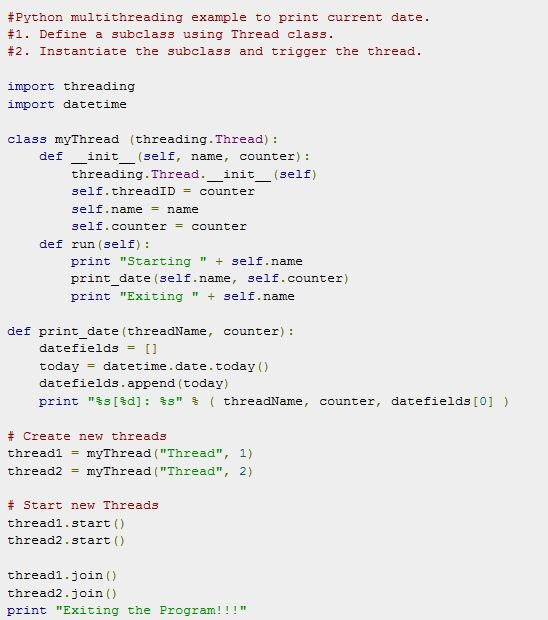
\includegraphics[width=0.75\textwidth]{figures/Thread}}
	\caption{Mengimplementasikan Thread menggunakan Threading}
	\label{Mengimplementasikan Thread menggunakan Threading}
\end{figure}

\chapter{XML Processing}

\chapter{GUI Programming}

\chapter{Futher Expression}


\begin{references}{3.}
\bibitem{kilby}J. S. Kilby,
``Invention of the Integrated Circuit,'' {\it IEEE Trans. Electron Devices,}
{\bf ED-23,} 648 (1976).

\bibitem{hamming}R. W. Hamming,
                 {\it Numerical Methods for Scientists and 
                 Engineers}, Chapter N-1, McGraw-Hill, 
                 New York, 1962.

\bibitem{Hu}J. Lee, K. Mayaram, and C. Hu, ``A Theoretical
               Study of Gate/Drain Offset in LDD MOSFETs''
                     {\it IEEE Electron Device Lett.,} {\bf EDL-7}(3). 152 
                     (1986).

\bibitem{beren}A. Berenbaum, 
B. W. Colbry, D.R. Ditzel, R. D Freeman, and 
K.J. O'Connor, ``A Pipelined 32b Microprocessor with 13 kb of Cache Memory,''
{it Int. Solid State Circuit Conf., Dig. Tech. Pap.,} p. 34 (1987).
\end{references}


\begin{references}{Ham62}
\bibitem[Kil76]{kilb}J. S. Kilby,
``Invention of the Integrated Circuit,'' {\it IEEE Trans. Electron Devices,}
{\bf ED-23,} 648 (1976).

\bibitem[Ham62]{hamm}R. W. Hamming,
                 {\it Numerical Methods for Scientists and 
                 Engineers}, Chapter N-1, McGraw-Hill, 
                 New York, 1962.

\bibitem[Hu86]{lee}J. Lee, K. Mayaram, and C. Hu, ``A Theoretical
               Study of Gate/Drain Offset in LDD MOSFETs''
                     {\it IEEE Electron Device Lett.,} {\bf EDL-7}(3). 152 
                     (1986).

\bibitem[Ber87]{berm}A. Berenbaum, 
B. W. Colbry, D.R. Ditzel, R. D Freeman, and 
K.J. O'Connor, ``A Pipelined 32b Microprocessor with 13 kb of Cache Memory,''
{it Int. Solid State Circuit Conf., Dig. Tech. Pap.,} p. 34 (1987).

\end{references}



%%%%%%%%%%%%%%%
%%  The default LaTeX Index
%%  Don't need to add any commands before \begin{document}
\printindex

%%%% Making an index
%% 
%% 1. Make index entries, don't leave any spaces so that they
%% will be sorted correctly.
%% 
%% \index{term}
%% \index{term!subterm}
%% \index{term!subterm!subsubterm}
%% 
%% 2. Run LaTeX several times to produce <filename>.idx
%% 
%% 3. On command line, type  makeindx <filename> which
%% will produce <filename>.ind 
%% 
%% 4. Type \printindex to make the index appear in your book.
%% 
%% 5. If you would like to edit <filename>.ind 
%% you may do so. See docs.pdf for more information.
%% 
%%%%%%%%%%%%%%%%%%%%%%%%%%%%%%

%%%%%%%%%%%%%% Making Multiple Indices %%%%%%%%%%%%%%%%
%% 1. 
%% \usepackage{multind}
%% \makeindex{book}
%% \makeindex{authors}
%% \begin{document}
%% 
%% 2.
%% % add index terms to your book, ie,
%% \index{book}{A term to go to the topic index}
%% \index{authors}{Put this author in the author index}
%% 
%% \index{book}{Cows}
%% \index{book}{Cows!Jersey}
%% \index{book}{Cows!Jersey!Brown}
%% 
%% \index{author}{Douglas Adams}
%% \index{author}{Boethius}
%% \index{author}{Mark Twain}
%% 
%% 3. On command line type 
%% makeindex topic 
%% makeindex authors
%% 
%% 4.
%% this is a Wiley command to make the indices print:
%% \multiprintindex{book}{Topic index}
%% \multiprintindex{authors}{Author index}

\end{document}

